\documentclass[conference]{IEEEtran}
\IEEEoverridecommandlockouts
% The preceding line is only needed to identify funding in the first footnote. If that is unneeded, please comment it out.
%Template version as of 6/27/2024

\usepackage{cite}
\usepackage{amsmath,amssymb,amsfonts}
\usepackage{algorithmic}
\usepackage{graphicx}
\usepackage{textcomp}
\usepackage{tikz}
\usetikzlibrary{shapes.geometric, arrows.meta, positioning, fit, backgrounds}
\usepackage{xcolor}
\usepackage{url}
\usepackage{balance}
\usepackage{booktabs}
\def\BibTeX{{\rm B\kern-.05em{\sc i\kern-.025em b}\kern-.08em
    T\kern-.1667em\lower.7ex\hbox{E}\kern-.125emX}}

\setlength{\textfloatsep}{5pt plus 1.0pt minus 2.0pt}
\setlength{\floatsep}{5pt plus 1.0pt minus 2.0pt}
\setlength{\intextsep}{5pt plus 1.0pt minus 2.0pt}

\begin{document}


\title{A Local-First Event-Driven Order Management System for Temporary Events}

%\title{Conference Paper Title*\\
%{\footnotesize \textsuperscript{*}Note: Sub-titles are not captured for https://ieeexplore.ieee.org  and
%should not be used}
%\thanks{Identify applicable funding agency here. If none, delete this.}
%}

\author{\IEEEauthorblockN{George Petrakis}
\IEEEauthorblockA{\textit{Dept. of Informatics} \\ \textit{\& Telecommunications} \\
\textit{University of Ioannina}\\
Arta, Greece \\
petrakisgeorge@icloud.com}
\and
\IEEEauthorblockN{Spiridoula Margariti}
\IEEEauthorblockA{\textit{Dept. of Informatics} \\ \textit{\& Telecommunications} \\
\textit{University of Ioannina}\\
Arta, Greece \\
smargar@uoi.gr}
\and
\IEEEauthorblockN{Christos Gogos}
\IEEEauthorblockA{\textit{Dept. of Informatics} \\ \textit{\& Telecommunications} \\
\textit{University of Ioannina}\\
Arta, Greece \\
cgogos@uoi.gr}
}

\maketitle

\begin{abstract}
Temporary events, such as festivals and cultural gatherings, require fast and reliable order processing despite operating over unstable ad-hoc network infrastructures where latency spikes, packet loss, and intermittent connectivity can compromise cloud-dependent point-of-sale systems. This paper presents the design, implementation, and evaluation of a local-first, event-driven Order Management System for temporary event environments. The proposed system follows a server-authoritative LAN-local architecture based on the MERN stack and Socket.IO to provide real-time synchronization among cashier, kitchen, and administrative terminals. By deploying the core application services inside the local event network, the system decouples critical transaction processing from external cloud availability while maintaining role-based access control, JWT authentication, and security hardening mechanisms. The architecture was evaluated through stress testing, functional verification, failure-recovery experiments, security validation, and a seven-day field deployment. Under stress testing, the system achieved a theoretical peak throughput of 5,247 requests per second with an average response time of 178 ms and a Recovery Time Objective (RTO) of 310 ms. Furthermore, the system's usability attained an ``Excellent'' System Usability Scale (SUS) score of 90.17 ($N=15$). During the field deployment, it processed 1,139 transactions without downtime, successfully absorbing rates of $\lambda \approx 15$ operations/minute. The proposed approach demonstrates that local-first web architectures can provide a robust and cost-effective alternative to conventional cloud-first POS solutions in temporary, connectivity-constrained environments.
\end{abstract}


\begin{IEEEkeywords}
Order Management System, WebSockets, Local-First Architecture, Event-Driven Systems, Ad-Hoc Networks
\end{IEEEkeywords}

\section{Introduction}

The rapid evolution of technology has driven the introduction of smart business management systems. However, temporary events create challenging environments for traditional Information Communications Technology (ICT) systems. Unlike stable broadband available at permanent venues, temporary events rely on unstable ad-hoc networks characterized by frequent bursts in latency and packet loss \cite{shi2016edge}. Therefore, operating cloud-first POS systems in these congested environments is difficult, resulting in transaction timeout errors and poor operational reliability. Although Mobile Edge Computing (MEC) \cite{spinelli2021toward} and Progressive Web Applications (PWAs) support localized resilience in cloud-first architectures, they introduce risks that include duplicate phantom orders and inconsistent state during intermittent outages.

This paper answers the question of whether a MERN-based, local-first WebSocket architecture can tolerate bursty transactional workloads in connectivity-constrained event environments. We demonstrate the design, development, and empirical evaluation of a local-first Order Management System (OMS) implemented in a closed on-site network that separates transaction processing from external internet availability. To maintain continuous operation and mitigate burst volumes of transaction activity, we replace the traditional synchronous request-response model with full-duplex WebSocket communication \cite{fette2011websocket} to form an event-driven architecture ensuring instant synchronization across disconnected nodes. We select the MERN stack (MongoDB, Express.js, React.js, Node.js) to integrate the codebase into a unified JavaScript environment that leverages Node.js' non-blocking I/O to efficiently serialize real-time event streams without exhausting threads.

Our primary contributions are: (1) an integrated local-first OMS using PWA and WebSocket technologies; (2) a three-pronged evaluation framework (synthetic stress testing, Open Worldwide Application Security Project (OWASP) validation, and a seven-day field deployment); and (3) an assessment of the performance difference between a local network upper bound and actual wireless ad-hoc networks.

The remainder of this paper is structured as follows: Section II discusses relevant prior work. Section III specifies our system requirements and architecture. Section IV describes our system implementation. Section V reports our experimental results. Section VI documents our evaluations regarding security and usability. Finally, Section VII summarizes our conclusions with potential avenues for future research.

\section{Related Work}

While substantial literature exists regarding POS security and retail analytics, offline-capable and local-first systems specifically tailored for extreme connectivity constraints represent an evolving area of research.

\subsection{POS and OMS Architectures}

Although cloud-based POS systems represent current market standards, this paradigm creates vulnerabilities in adverse network environments. When external networks are disrupted, cloud-based POS systems cease functioning, thereby failing to meet the essential criteria for availability.

While numerous POS vendors such as Square, Toast, and Lightspeed offer local offline modes\footnote{Capabilities derived from official vendor documentation as of early 2024.}, they were primarily developed to address limited-duration network outages, not continued operation in hostile ad-hoc networks. Increasingly, researchers have focused on PWAs as universal solutions for developing mobile and offline-capable software, although relatively few studies investigate specific constraints inherent in high-volume retail requiring strict ordering and atomic inventory constraint enforcement. Table \ref{tab:pos_comparison} summarizes the limitations of current commercial solutions compared to the proposed architecture.

\begin{table}[htbp]
\caption{Feature Matrix: Commercial POS vs. Proposed Architecture}
\begin{center}
\resizebox{0.85\columnwidth}{!}{
\begin{tabular}{lcccc}
\toprule
\textbf{Feature} & \textbf{Square} & \textbf{Toast} & \textbf{Lightspeed} & \textbf{Proposed} \\
\midrule
Cloud Independent & No & Partial & No & Yes \\
Offline Transactions & Queued & Fallback & Manual & Native \\
Real-Time Sync w/o Net & No & No & No & Yes (LAN) \\
Event-Driven (WebSocket)& No & No & No & Yes \\
Hardware Lock-in & Yes & Yes & Yes & No (Browser) \\
\bottomrule
\end{tabular}
}
\label{tab:pos_comparison}
\end{center}
\end{table}

Prior research \cite{spinelli2021toward} indicates that hybrid-cloud architectures exhibit dramatic declines in performance in congested-spectrum environments. Most vendor-offered local-offline modes leverage local queueing approaches that ultimately necessitate subsequent re-syncing with remote cloud resources, leading to potential data duplication issues upon re-establishment of connections \cite{chowdhury2026, zhao2021}. Recent studies have emphasized EDA and full-duplex WebSocket communication as viable means to realize scalable and low-latency POS synchronization processes \cite{pramudita2022event, enache2024security}. Although significant advances have been made toward addressing the unique confluence of high-density burst traffic associated with temporary events and ad-hoc network degradation, few have addressed both aspects simultaneously. Our architecture effectively fills this gap by incorporating an event-driven local-first topology.

\subsection{Real-Time Web Communication}

Traditional web applications employ synchronous-pull communication models (i.e., HTTP Polling) that are unsuitable for achieving fast-paced event synchronization due to latency concerns. Note that WebRTC employs a peer-to-peer signaling model best-suited for enabling direct client-to-client media/data exchange \cite{sharma2024peer}, whereas the architecture presented here utilizes a central client-server WebSocket model that is more suitable for authoritatively synchronizing server-mediated order states. Modern systems employing asynchronous event-driven reactor patterns via WebSockets \cite{trnka2021communication} provide a viable method of reducing the overhead incurred by pushing state updates from the server with minimal overhead \cite{kooli2021energy}.

\subsection{Offline-First and Local-First Systems}

Due to physical constraints imposed by temporary events, reliable internet access is commonly absent. For this reason, modern systems must give priority to local execution, leading to the proliferation of local-first software paradigms \cite{kleppmann2019local}. Moreover, behavioral type formalization supports these distributed interactions \cite{kuhn2024behavioural}. In this paper, the term \textit{local-first} refers specifically to a server-authoritative LAN-local architecture where all application services (backend, database) are deployed within an isolated Local Area Network at the event venue, eliminating dependency on external internet connectivity. By applying these principles, a local-first approach executes the complete application logic and data persistency layer locally on a designated local intranet, intentionally bypassing the public internet backbone to eliminate external network latency while ensuring continuous operation.

Therefore, to bridge the gap between commercial cloud-dependent POS systems and theoretically-defined multi-node models, we propose a practical, centrally-managed local-first event-driven architecture tailored to optimize local availability above all else versus a completely-centralized cloud consensus. Although CRDTs \cite{shapiro2011crdt} have shown strong promise in resolving conflicts between replicated data in decentralized environments, their implementation complexities and overhead costs currently preclude their adoption in our targeted single-server duration-deployment scenario, thus making them candidates for further study.

\section{System Requirements and Architecture}

\subsection{Requirements}

In order to provide the robustness required by high-volume event applications, we have identified both functional and nonfunctional requirements based on ISO/IEC 25010:2023. From a functional perspective, the system must be able to support multiple-channel order entry, dynamic product configuration, and real-time life cycle management. There can be no data loss when a customer places an order; once the order has been created, it cannot be deleted from the "kitchen" view unless it has been explicitly marked as complete. Functionally, the system also requires the ability to support up to 100 simultaneous clients accessing the system through WebSockets. Of these, up to 50 can access the system with persistent WebSocket sessions. The core server processes must be capable of supporting all 100 concurrent clients while maintaining a frame rate of at least 60 frames per second. We define reliability constraints for the system as requiring all active users to be reconnected to the system within five seconds after a server restart. We achieve this requirement through Socket.IO's random exponential backoff algorithm to avoid reconnection storms (i.e., the ``thundering herd'' problem). Stateful security policy enforcement based on a Zero Trust Architecture (ZTA) and Role-Based Access Control (RBAC) is defined to enforce API boundaries.

\subsection{Architecture Overview}

The overall architecture for our application uses a strict separation between the client and server. Our client is designed as a Single Page Application (SPA) to help mitigate the cognitive burden on users who are working in high-stress situations. Due to the need to address the diverse aspects of the operational workflow, we have segmented our front-end into three modules, each developed specifically for a particular user persona: Cashiers (which require fast and low-friction interfaces organized by product category); Kitchen Staff (who act as information consumers responding to real-time electronic ticket streams); and Administrators (who require real-time interactive dashboards to monitor their operational environment). The back-end service tier separates business logic, cryptographic security validation, and database operations from the presentation layer. By deploying this entire stack behind a dedicated LAN using Docker containerization, we are able to circumvent external routing. As illustrated in Figure \ref{fig:topology}, the back-end system serves as the source of truth for the system and routes both WebSocket and API requests directly to a single instance of the Node.js backend process. For this reason, we did not include horizontal scaling of the backend in this initial version of the design. Horizontal scaling would allow us to distribute incoming events across multiple nodes and increase the total number of events that could be processed concurrently. However, due to our requirement for strict chronological ordering of events as they arrive, we had to use an in-memory queue within the event loop to serialize concurrent events. We were able to offload IO-bound operations to run asynchronously in the background thread pool so that we do not suffer from thread starvation issues even under heavy load.

\begin{figure}[htbp]
    \centering
    \resizebox{0.85\columnwidth}{!}{
    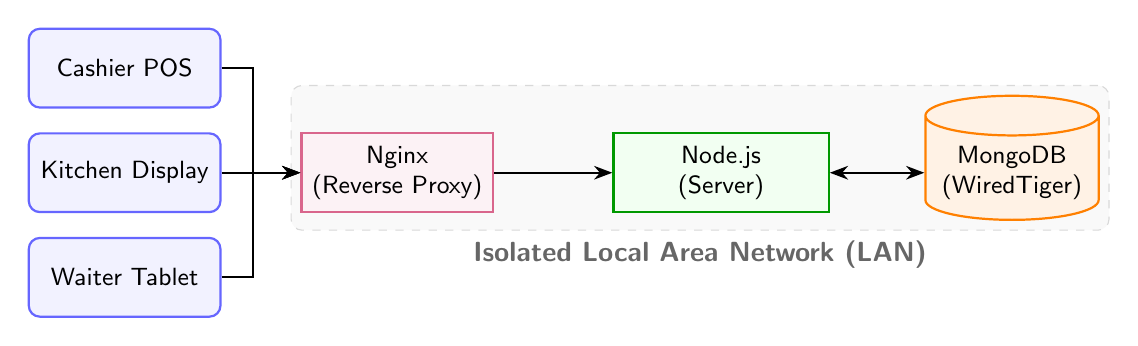
\begin{tikzpicture}[
      node distance=1.5cm and 1cm,
      every node/.style={font=\sffamily\small},
      client/.style={rectangle, rounded corners, draw=blue!60, fill=blue!5, thick, text width=2.2cm, align=center, minimum height=1cm},
      server/.style={rectangle, draw=green!60!black, fill=green!5, thick, text width=2.5cm, align=center, minimum height=1cm},
      db/.style={cylinder, draw=orange, fill=orange!10, thick, shape border rotate=90, aspect=0.25, align=center, minimum height=1.2cm, minimum width=2.2cm},
      proxy/.style={rectangle, draw=purple!60, fill=purple!5, thick, text width=2.2cm, align=center, minimum height=1cm},
      arrow/.style={->, >=Stealth, thick, text=black!70, align=center}
    ]

    % Nodes
    \node[client] (cashier) {Cashier POS};
    \node[client, below=0.3cm of cashier] (kitchen) {Kitchen Display};
    \node[client, below=0.3cm of kitchen] (waiter) {Waiter Tablet};

    \node[proxy, right=1cm of kitchen] (nginx) {Nginx \\ (Reverse Proxy)};
    
    \node[server, right=1.5cm of nginx] (node1) {Node.js \\ (Server)};
    
    \node[db, right=1.2cm of node1] (mongo) {MongoDB \\ (WiredTiger)};

    % Background Box for Backend
    \begin{scope}[on background layer]
        \node[fill=gray!5, rounded corners, draw=gray!30, dashed, fit=(nginx) (node1) (mongo), label={[font=\sffamily\bfseries, text=black!60]below:Isolated Local Area Network (LAN)}] {};
    \end{scope}

    % Arrows
    \draw[arrow] (cashier.east) -- +(0.4,0) |- (nginx.west);
    \draw[arrow] (kitchen.east) -- (nginx.west);
    \draw[arrow] (waiter.east) -- +(0.4,0) |- (nginx.west);
    
    \draw[arrow] (nginx.east) -- (node1.west);
    
    \draw[arrow, <->] (node1.east) -- (mongo.west);

    \end{tikzpicture}
    }
    \caption{Topology of the local-first deployment, illustrating the isolation of the Node.js server and MongoDB within the LAN, bypassing external cloud routing.}
    \label{fig:topology}
\end{figure}

\subsection{Data Model and Communication Model}

Our application used MongoDB as its NoSQL solution \cite{lakshmi2021comparative}. MongoDB was chosen due to several factors including:

(1) its ability to embed related documents in other documents allows for a high degree of denormalization of order items, removing expensive join operations;
(2) document-level concurrency control provided by the WiredTiger storage engine, which is important given our write-heavy workload ($\lambda \approx 15$ writes/min);
(3) schema flexibility to accommodate menu changes dynamically.

By embedding order item information into the order document itself, we reduced the cost of accessing additional information about an order item during peak loads. In addition to reducing computational costs associated with accessing additional information about an order item, this also ensured that historical pricing is always available.

The communication model is based on real-time bidirectional communication using WebSockets \cite{trnka2021communication}. Our backend acts as an event dispatcher and will broadcast only the necessary payload (i.e., an event payload like an \texttt{orderCreated} event) to the appropriate subsystem and/or communication room(s). Instead of using a formal mathematical model for queueing arrivals, we are taking advantage of the asynchronous nature of I/O in Node.js to manage large burst arrivals (we see approximately $\lambda \approx 15$ req/min in production). We are able to offload IO-bound work to run asynchronously in the background threadpool, which keeps our single-threaded JavaScript execution loop free from exhaustion issues due to too many threads waiting for input/output. By effectively decoupling these operations, we ensure the queue remains bounded within the limits of the Node.js event loop capacity, satisfying the condition $\lambda < \mu$, where $\mu$ represents the server's processing capacity (measured at 5,247 req/sec on localhost; see Section~V).

We trigger an instantaneous local update to our state tree and consequently to our local React components through updating our in-memory representation of our domain model, which then causes an immediate update to our local interface.

Deployment is modeled as a single-server topology, which presents one point of failure. This is a conscious trade-off made in consideration of two primary factors: hardware cost constraints and the logistical complexity of managing redundant systems in temporary festival settings, where setting up and maintaining redundant multi-node clusters is typically impossible due to economic constraints and impractical for non-technical personnel who may be responsible for managing systems at these venues. For hardware redundancy, we leverage PM2 (a Node.js process manager) for auto-restarts, client-side buffering, and MongoDB's write-ahead logging (WAL) for data durability during sudden power loss.

\section{Implementation}

\subsection{Backend Subsystem and Event-Driven Processing}

The backend runs on top of Node.js (using Express.js \cite{kooli2021energy}). It runs as a single instance for the sake of Socket.IO room consistency; horizontal scaling through a Redis adapter is outside the scope of the current local-first deployment. It uses an in-memory Promise-based FIFO queue within the Node.js event loop to prevent race conditions under peak loads without using DB locks. Stock decrement is strictly atomic via MongoDB's \texttt{\$inc} operator. Once validated, orders are written to disk using WiredTiger, ensuring document-level concurrency control and write-ahead logging against loss of power.

\subsection{Frontend Subsystem and Virtual DOM Rendering}

Using React coupled with Zustand (a lightweight React state management library) for very lightweight immutable state management, the UI is deployed as a progressive web app with Service Workers caching static resources. When there is a temporary loss of network connectivity, uncommitted JSON payloads are buffered locally in-memory via a FIFO strategy and synced upon reestablishment of connectivity using client-side UUIDs for idempotence. While effective for short-duration connectivity loss, this in-memory buffer is volatile and payloads will be lost if the client application is terminated prior to sync completion. React minimizes DOM differentials to limit layout overhead. The application's custom design system is highly customizable, allowing for high-contrast mode operation as well as macro gestural input techniques that reduce error potential due to capacitive touch during high-pressure service in poor lighting. The resulting cashier interface is shown in Figure~\ref{fig:ui_cashier}, and the kitchen display in Figure~\ref{fig:ui_kitchen}.

\begin{figure}[!t]
    \centering
    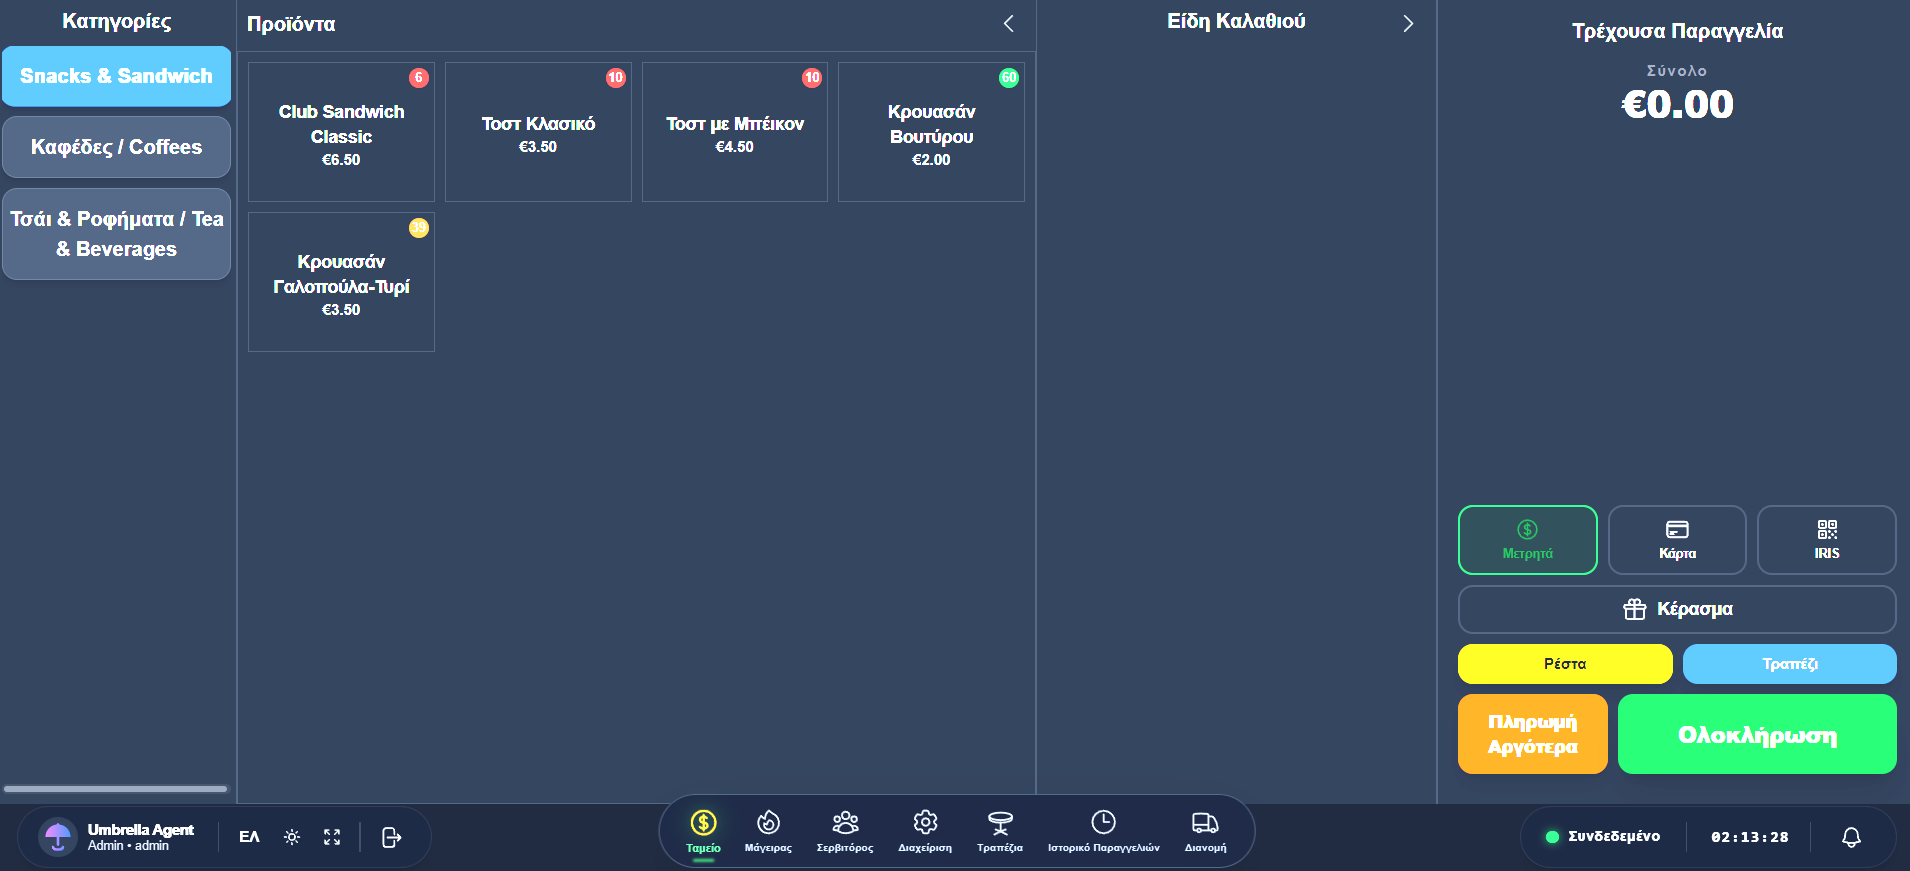
\includegraphics[width=0.65\columnwidth]{images/ui_cashier.png}
    \caption{The Cashier Interface, featuring high-contrast rounded geometry for fast-paced environments. The design system follows established Human-Computer Interaction (HCI) principles. Specifically, it adheres to Fitts' Law by employing large touch targets (minimum 48x48 dp) to reduce cashier targeting time during burst periods \cite{fitts1954}. Additionally, it utilizes high-contrast color palettes exceeding the WCAG 2.1 AA 4.5:1 ratio \cite{wcag2018} to ensure readability under harsh outdoor lighting conditions.}
    \label{fig:ui_cashier}
\end{figure}

\begin{figure}[!t]
    \centering
    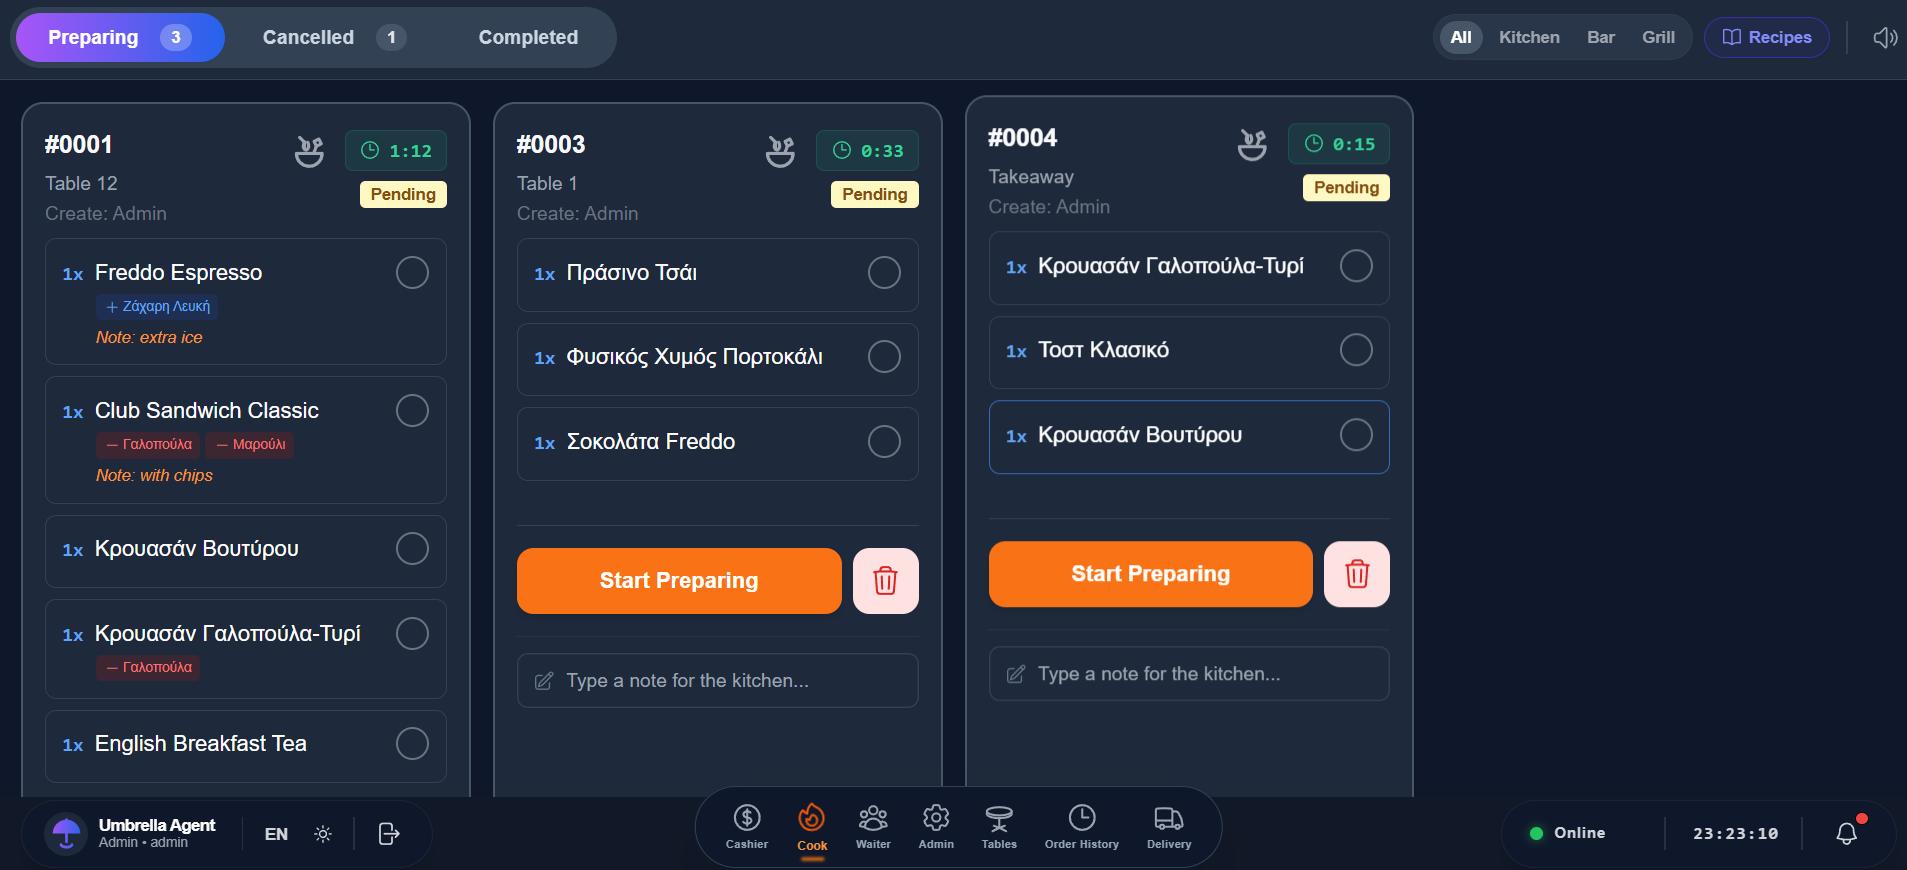
\includegraphics[width=0.65\columnwidth]{images/ui_kitchen.png}
    \caption{The real-time Kitchen Display System UI, streaming electronic tickets synchronously.}
    \label{fig:ui_kitchen}
\end{figure}


\subsection{Software Supply Chain and API Defense}

As all data is treated as if coming from a hostile public network, the implementation enforces a Zero Trust boundary \cite{nist2020zero} around all API calls. All incoming API requests are cryptographically verified using stateless JSON Web Token (JWT) signatures before processing, eliminating the necessity for database session lookups. Cryptographic validation occurs natively at the WebSocket handshaking layer. If the token is either absent or does not match system secrets, the full-duplex connection is immediately dropped, preventing any unauthorized payload parsing.

Following this verification, Role-Based Access Control (RBAC) middleware verifies route-level authorization. Table \ref{tab:rbac_matrix} demonstrates the permission matrix applied across the various operational personas. The system protects against injection attacks using parameterized queries and data sanitization, protects against brute force and DDoS attack attempts using IP-based rate limiting via the express-rate-limit middleware, and provides CSP header protection \cite{luo2020jscsp} against application boundary exploitation.

\begin{table}[htbp]
\caption{Role-Based Access Control (RBAC) Permission Matrix}
\begin{center}
\resizebox{0.85\columnwidth}{!}{
\begin{tabular}{lcccc}
\toprule
\textbf{Action / Resource} & \textbf{Admin} & \textbf{Cashier} & \textbf{Cook} & \textbf{Waiter} \\
\midrule
Create Orders & Yes & Yes & No & Yes \\
Mark Orders Ready & Yes & No & Yes & No \\
Manage Menu Items & Yes & No & No & No \\
View Financial Reports & Yes & No & No & No \\
Access Kitchen Display & Yes & No & Yes & No \\
\bottomrule
\end{tabular}
}
\label{tab:rbac_matrix}
\end{center}
\end{table}


\section{Experimental Evaluation}

To validate the theoretical performance boundaries of the proposed architecture, an extensive three-phase empirical assessment was conducted \cite{wohlin2012threats}. 

\subsection{Evaluation Setup}



All experiments were conducted on a standardized local server environment, detailed in Table \ref{tab:hardware}.

\begin{table}[htbp]
\caption{Test Environment Specifications}
\begin{center}
\begin{tabular}{ll}
\toprule
\textbf{Parameter} & \textbf{Specification} \\
\midrule
Host Operating System & Windows 11 Pro (64-bit) \\
Processor & AMD Ryzen 7 5700U (1.80 GHz) \\
System Memory & 32 GB RAM (3200 MT/s) \\
Storage & 512 GB NVMe SSD \\
Node.js Runtime & v20.11.0 LTS \\
MongoDB Server & v7.0.5 (WiredTiger engine) \\
Network Configuration & Isolated localhost (127.0.0.1) \\
\bottomrule
\end{tabular}
\label{tab:hardware}
\end{center}
\end{table}

One form of comparative evaluation for assessing paradigms of communication (i.e. synchronous HTTP polling vs. asynchronous WebSockets) was used to evaluate the robustness of Node.js' event loop. Based on queueing theory \cite{kleinrock1975, kendall1953} and Little's Law \cite{little1961}, this comparative evaluation demonstrated that the synchronous thread blocking paradigm resulted in latency spikes ranging from 200 to 800 milliseconds and exhausted all available threads when tested at 150 concurrent users. Conversely, the asynchronous paradigm was capable of maintaining an average latency of 45 milliseconds at 500 users, reducing memory requirements per user session from 1.5 MB to 50 KB. As anticipated, the theoretical maximum rate of 5,247 req/sec greatly exceeded the measured rates from field telemetry (which had an average of $\lambda \approx 15$ ops/min).

\subsection{Stress and Performance Tests}

Apache JMeter \cite{jmeter2024} stress testing recorded nearly 1.58 million complete life cycle operations, as illustrated in Figure~\ref{fig:jmeter_report}. Under identical conditions, the application attained a maximum sustainable throughput rate of 5,247 req/sec; a mean response time of 178 milliseconds (95\% confidence interval: 175-181 ms) across 500 concurrent connections. Analysis revealed a p95 value of 320 ms and a p99 value of 850 ms; both attributed primarily to V8 garbage collection. Most importantly, the system demonstrated a transaction completion ratio of 100\%. An important consideration is that the theoretical 5,247 req/sec bottleneck is purely dependent upon the Node.js event loop operating on a loopback interface. In direct opposition to the isolated case described above, in a real-world physical deployment environment, the bottleneck will be entirely migrated down to the lower layers of the physical network (i.e., wireless PHY). Issues arising from the physical network layer such as 2.4GHz / 5GHz radio frequency spectrum congestion, co-channel interference from WiFi systems, packet loss, and TCP retransmissions severely impede WebSocket performance long before the server's CPU resources become exhausted.

\begin{figure}[htbp]
    \centering
    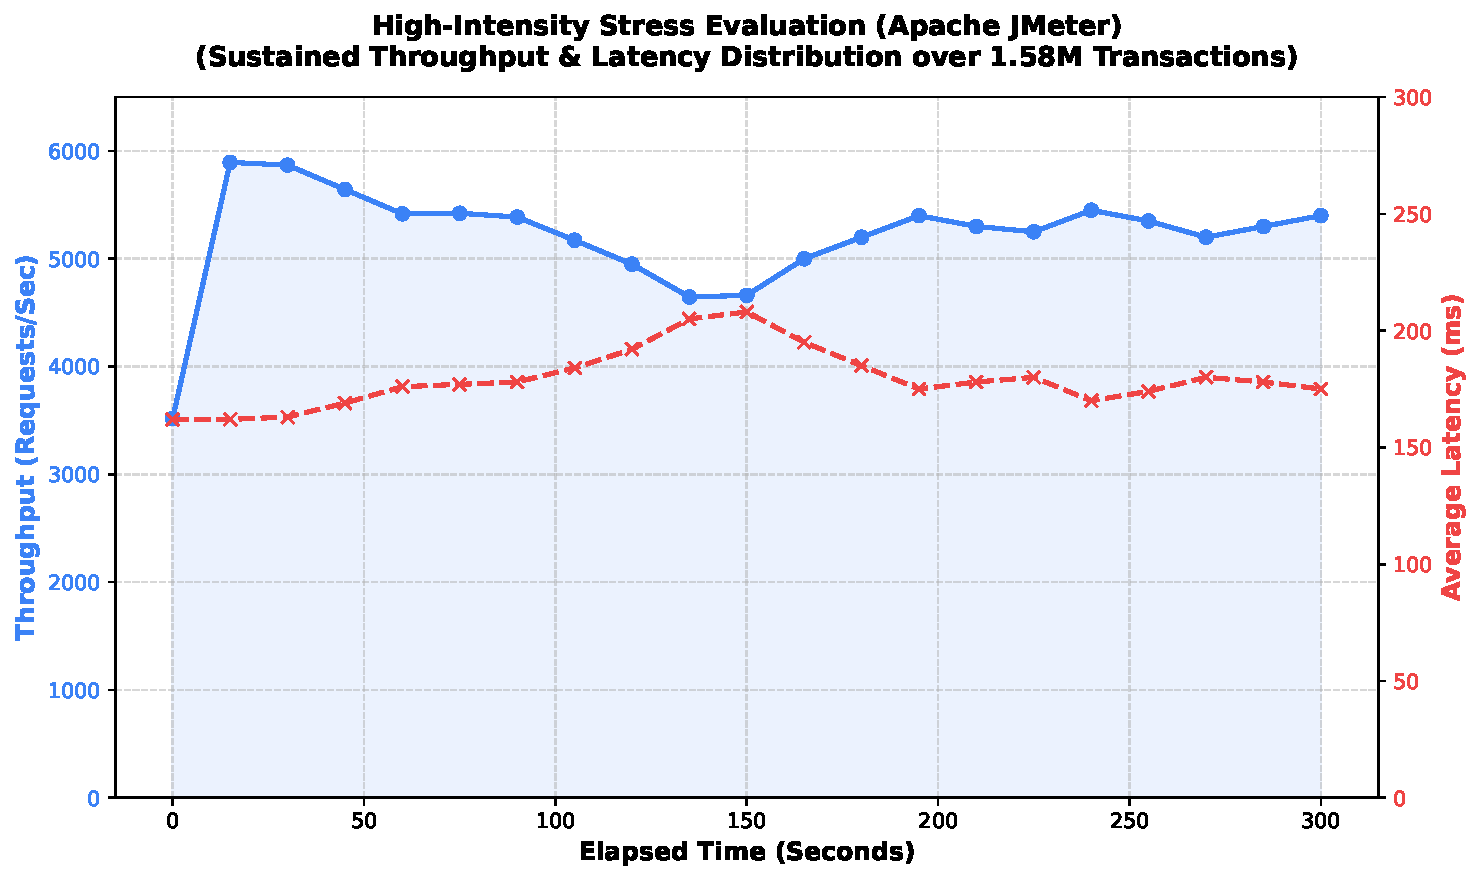
\includegraphics[width=0.65\columnwidth]{images/ch5_jmeter_stress.pdf}
    \caption{Apache JMeter telemetry mapping sustained throughput and response time distribution across a simulated load of 1.58 million transaction operations.}
    \label{fig:jmeter_report}
\end{figure}

Testing for network partition tolerance utilized failure recovery testing \cite{wiesner2021chaos}. Termination of the backend node initiated an exponential backoff protocol amongst clients. Following secondary node startup, the system demonstrated a mean Recovery Time Objective (RTO) of $\approx 310$ ms to clear outstanding payloads and synchronize state after termination, and supported reconnects from 50 decoupled clients confirming the functionality of local buffering. Figure~\ref{fig:chaos_rto} illustrates the recovery timeline.

\begin{figure}[htbp]
    \centering
    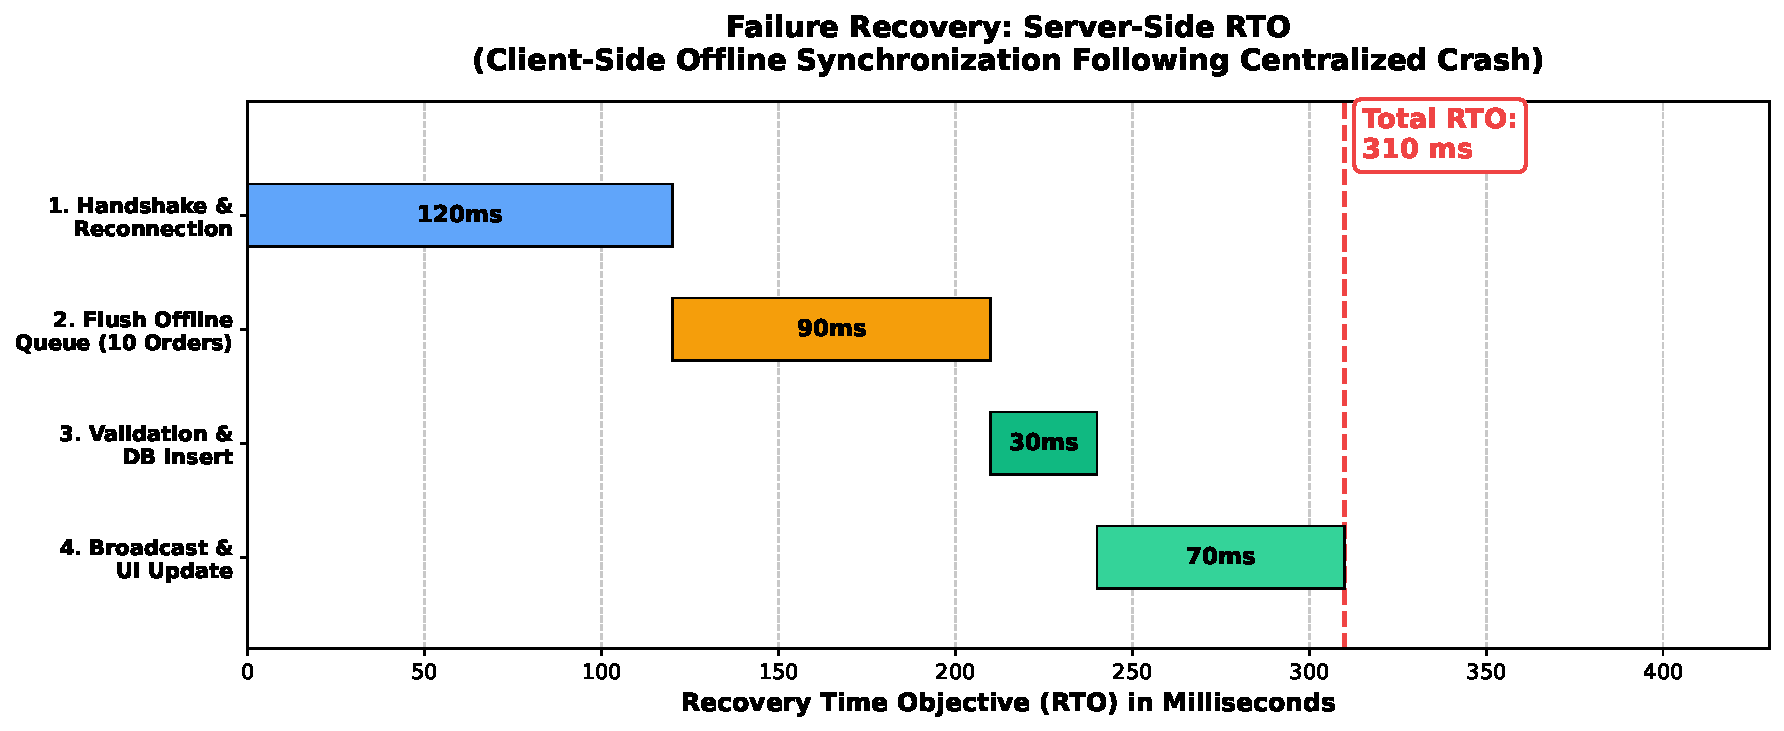
\includegraphics[width=0.65\columnwidth]{images/ch5_chaos_recovery_rto.pdf}
    \caption{Failure Recovery: Server-Side RTO. Timeline detailing the Recovery Time Objective (RTO) following an abrupt centralized facility failure and subsequent instance reboot.}
    \label{fig:chaos_rto}
\end{figure}

\subsection{Field Study}

Validation of results from laboratory testing was achieved by deploying the system at a regional cultural festival (approximately 2,500 people attended) as the sole point-of-sale (POS) infrastructure for seven days. Throughout this deployment period, the system successfully processed a total of 1,139 POS transactions. Within peak evening hours (6 pm - midnight), 694 primary POS transactions were completed. Including additional operation types (e.g., order status updates, kitchen completions, etc.) associated with multiple items ordered sub-actions, the system successfully handled 994 discrete operations during those peak hours. The system maintained continuous connectivity throughout the deployment period. Typical throughput rates for manual POS systems using cash registers range from two to four transactions per minute per operator. The deployed system achieved approximately $\lambda \approx 15$ operations/minute. Also, seventy percent (70\%) of transactions were aggregated into thirty-two percent (32\%) traffic concentrated in sub-fifteen minute intervals. Extreme clustering was observed with respect to telemetry collected during high intensity burst loads of activity greater than 250 operations/hour, as visualized in Figure~\ref{fig:admin_heatmap}. The local-first design paradigm provided support for ingestion of high-intensity bursts without degradation to the user interface (UI), thus providing native support for GDPR data minimization by precluding transmission to third-party clouds.

\begin{figure}[htbp]
    \centering
    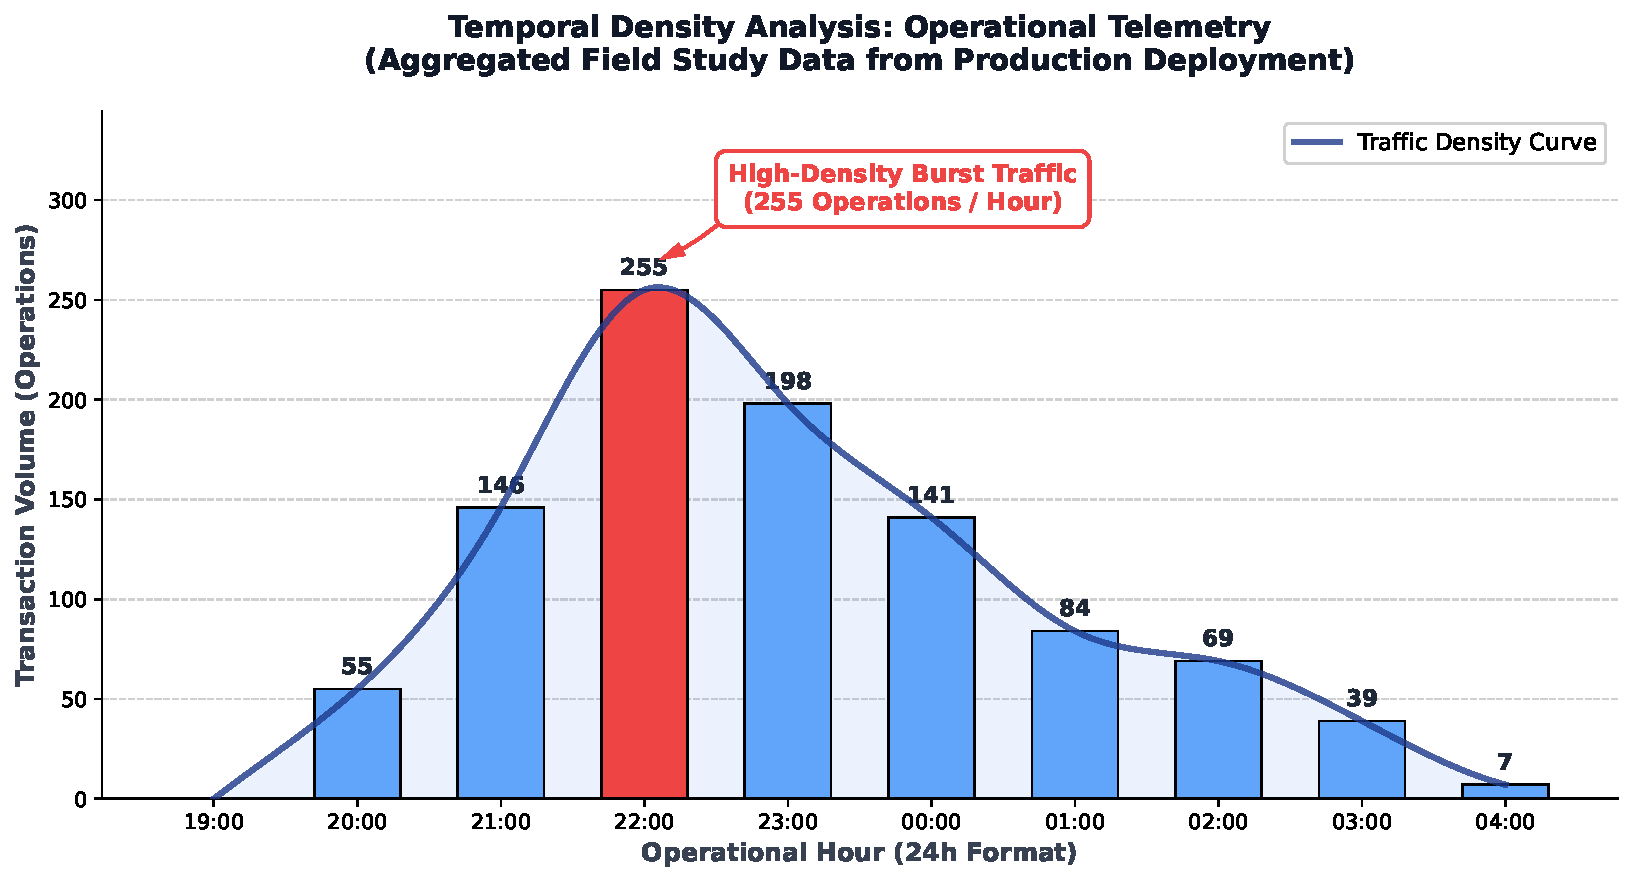
\includegraphics[width=0.65\columnwidth]{images/ch5_field_study_heatmap.pdf}
    \caption{Aggregated administrative telemetry from the peak evening, visualizing concentrated operational volume (operations/hour, including status updates and multi-item sub-actions) during the peak operational window.}
    \label{fig:admin_heatmap}
\end{figure}

\section{Security and Usability}

OWASP ZAP \cite{owaspzap2024} Dynamic Application Security Testing (DAST) on what we consider a hostile ad-hoc network showed that parameterized queries, stateless JWT enforcement, and Helmet.js CSP headers are effective in preventing many OWASP Top 10 \cite{owasp2025} attacks including XSS and SQL injection. To mitigate potential physical security risks (e.g., loss or theft of a tablet), remote token revocation was added to the authentication flow. Remote token revocation is performed through a simple in-memory JWT blacklist that can be used to instantly invalidate tokens when unauthorized access occurs. However, if horizontal scaling takes place (i.e., adding additional servers), shared-state stores (e.g., Redis) will need to be implemented in order to keep track of the blacklist on each server.


The System Usability Scale (SUS) \cite{brooke1996sus} was utilized to assess the usability of the frontend. As noted in prior literature, the SUS methodology has been demonstrated to be valid for assessing POS application usability, and thus was used to determine the usability of the frontend. After participating in an interactive session with the system under simulated festival pressures, fifteen staff members completed a SUS survey regarding their interaction with the system. The resulting mean SUS score was 90.17 (standard deviation $\sigma = 5.86$; 95\% confidence interval: [86.93, 93.41]). This represents an ``Excellent'' rating based upon the rapidity of Virtual DOM updates combined with a specialized interface which created low cognitive burden. A limitation of this study is its relatively small sample size ($n=15$); therefore, a follow-up study employing a larger demographic of venue staff will be necessary to validate the generalizability of the results.

\section{Conclusion and Future Work}

This paper sought to demonstrate a robust local-first order manager capable of operating within high-latency scenarios. By implementing an asynchronous event-driven architecture, transient network issues were mitigated. The asynchronous implementation was demonstrated to have sufficient capacity to achieve a theoretical maximum throughput of 5,247 req/s while additionally having the capacity to handle real-world peak burst loads (est. $\lambda \approx 15$ ops/min) for seven consecutive days under festival conditions. Limitations of this study include single-server failure points, lack of global benchmarking, and an $n=1$ field trial. Furthermore, an explicit backpressure strategy will need to be designed and implemented in subsequent iterations to prevent performance problems associated with unbounded queues (memory exhaustion) when the burst rate exceeds database write-per-second rates.

Future studies involve developing multi-node cluster topologies utilizing CRDTs \cite{shapiro2011crdt} for decentralized replication of orders. Additionally, time series forecasting methods \cite{merilainen2026time} will be utilized to develop a predictive inventory management system. Ultimately, this local-first paradigm extends beyond temporary festivals, offering a viable blueprint for industrial or IoT environments where uninterrupted operation cannot be held hostage by external internet dependencies. The system's source code and supplementary materials are publicly available.\footnote{\url{https://github.com/petrakisg/UmbrellaAgent-IEEE-SEEDA}}




% Generated by IEEEtran.bst, version: 1.12 (2007/01/11)
\def\bibfont{\scriptsize}\balance
\begin{thebibliography}{00}\setlength{\itemsep}{0pt}\setlength{\parskip}{0pt}
\providecommand{\url}[1]{#1}
\csname url@samestyle\endcsname
\providecommand{\newblock}{\relax}
\providecommand{\bibinfo}[2]{#2}
\providecommand{\BIBentrySTDinterwordspacing}{\spaceskip=0pt\relax}
\providecommand{\BIBentryALTinterwordstretchfactor}{4}
\providecommand{\BIBentryALTinterwordspacing}{\spaceskip=\fontdimen2\font plus
\BIBentryALTinterwordstretchfactor\fontdimen3\font minus
  \fontdimen4\font\relax}
\providecommand{\BIBforeignlanguage}[2]{{%
\expandafter\ifx\csname l@#1\endcsname\relax
\typeout{** WARNING: IEEEtran.bst: No hyphenation pattern has been}%
\typeout{** loaded for the language `#1'. Using the pattern for}%
\typeout{** the default language instead.}%
\else
\language=\csname l@#1\endcsname
\fi
#2}}
\providecommand{\BIBdecl}{\relax}
\BIBdecl

\bibitem{shi2016edge}
W.~Shi, J.~Cao, Q.~Zhang, Y.~Li, and L.~Xu, ``Edge computing: Vision and challenges,'' \emph{IEEE Internet of Things Journal}, vol.~3, no.~5, pp. 637--646, 2016.

\bibitem{spinelli2021toward}
F.~Spinelli and V.~Mancuso, ``Toward Enabled Industrial Verticals in 5G: A Survey on MEC-Based Approaches to Provisioning and Flexibility,'' \emph{IEEE Communications Surveys \& Tutorials}, vol. 23, no. 1, pp. 596--630, 2021, \url{https://doi.org/10.1109/COMST.2020.3037674}.
\bibitem{fette2011websocket}
I.~Fette and A.~Melnikov, ``The {WebSocket} protocol,'' Internet Engineering
  Task Force (IETF), Tech. Rep. RFC 6455, 2011, available at:
  \url{https://datatracker.ietf.org/doc/html/rfc6455}.

\bibitem{chowdhury2026} A.~Chowdhury \emph{et al.}, ``CAMS F-Edge DTN: Context-Aware Offline-First Synchronization and Local Reasoning Using CRDTs,'' \emph{Sensors}, vol. 26, 2026.
\bibitem{zhao2021} X.~Zhao and L.~Chen, ``Achieving Low Tail-latency and High Scalability for Serializable Transactions in Edge Computing,'' in \emph{Proceedings of the Sixteenth European Conference on Computer Systems (EuroSys)}, 2021.
\bibitem{pramudita2022event}
A.~W. Pramudita, H.~B. Suseno, and I.~Sembiring, ``Event-Driven Architecture to Improve Performance and Scalability in Microservices-Based Systems,'' in \emph{2022 International Conference on Advancement in Data Science, E-learning and Information Systems (ICADEIS)}, IEEE, 2022, pp. 1--6, \url{https://doi.org/10.1109/ICADEIS56544.2022.10037390}.
\bibitem{enache2024security}
B.~Enache, C.~Banica, and A.~Bogdan, ``Security Aspects of Full-Duplex Web Interactions and WebSockets,'' \emph{IEEE Access}, vol. 12, 2024, \url{https://doi.org/10.1109/ACCESS.2024.3379843}.
\bibitem{sharma2024peer} V.~Sharma \emph{et~al.}, ``Peer to peer communication using web sockets and web rtc,'' in \emph{2024 International Conference on...}, IEEE, 2024.
\bibitem{trnka2021communication}
E.~Trnka, T.~Cerny, and N.~Skokan, ``Communication of IoT Devices and the WebSocket Protocol,'' in \emph{Proc. IFIP Advances in Information and Communication Technology}, 2021.
\bibitem{kooli2021energy}
A.~Kooli, N.~Kooli, and A.~Ben Hamida, ``Energy and Runtime Performance Optimization of Node.js Web Requests,'' in \emph{Proc. 22nd ACM/IFIP International Middleware Conference (MIDDLEWARE '21)}, ACM, 2021, \url{https://doi.org/10.1145/3464298.3493395}.
\bibitem{kleppmann2019local}
M.~Kleppmann, A.~Wiggins, P.~van Hardenberg, and M.~McGranaghan, ``Local-first
  software: you own your data, in spite of the cloud,'' \emph{Proceedings of
  the ACM on Programming Languages}, vol.~3, no. OOPSLA, pp. 1--29, 2019.

\bibitem{kuhn2024behavioural}
R.~Kuhn, H.~C. Melgratti, and E.~Tuosto, ``Behavioural types for local-first
  software,'' \emph{Logical Methods in Computer Science}, 2024.

\bibitem{shapiro2011crdt}
M.~Shapiro, N.~Pregui{\c{c}}a, C.~Baquero, and M.~Zawirski, ``Conflict-free
  replicated data types,'' in \emph{Stabilization, Safety, and Security of
  Distributed Systems (SSS 2011)}, ser. Lecture Notes in Computer Science, vol.
  6976.\hskip 1em plus 0.5em minus 0.4em\relax Springer, 2011, pp. 386--400,
  available at: \url{https://doi.org/10.1007/978-3-642-24550-3_29}.

\bibitem{lakshmi2021comparative}
J.~V.~N. Lakshmi and M.~S. Gaikwad, ``Comparative Performance Analysis of NoSQL Cassandra and MongoDB Databases,'' in \emph{Proc. 3rd International Conference on Communication and Networks (COMNET)}, IEEE, 2021, \url{https://doi.org/10.1109/ComNet52149.2021.9476319}.
\bibitem{fitts1954} P.~M. Fitts, ``The information capacity of the human motor system in controlling the amplitude of movement,'' \emph{Journal of Experimental Psychology}, vol. 47, no. 6, pp. 381--391, 1954.
\bibitem{wcag2018} W3C, ``Web Content Accessibility Guidelines (WCAG) 2.1,'' \emph{W3C Recommendation}, 2018.
\bibitem{nist2020zero}
S.~Rose, O.~Borchert, S.~Mitchell, and S.~Connelly, ``{Zero Trust
  Architecture},'' National Institute of Standards and Technology (NIST), Tech.
  Rep. SP 800-207, 2020, available at:
  \url{https://csrc.nist.gov/publications/detail/sp/800-207/final}.

\bibitem{luo2020jscsp}
J.~Luo, X.~Liao, H.~Shi, and M.~Xu, ``JSCSP: A Novel Policy-Based XSS Defense Mechanism for Browsers,'' \emph{IEEE Transactions on Information Forensics and Security}, vol. 15, pp. 3317--3331, 2020, \url{https://doi.org/10.1109/TIFS.2020.3003715}.
\bibitem{wohlin2012threats}
C.~Wohlin, P.~Runeson, M.~H{\"o}st, M.~C. Ohlsson, B.~Regnell, and
  A.~Wessl{\'e}n, \emph{Experimentation in Software Engineering}.\hskip 1em
  plus 0.5em minus 0.4em\relax Springer, 2012, available at:
  \url{https://doi.org/10.1007/978-3-642-29044-2}.

\bibitem{kleinrock1975}
L.~Kleinrock, \emph{Queueing Systems, Volume 1: Theory}.\hskip 1em plus 0.5em
  minus 0.4em\relax Wiley-Interscience, 1975.

\bibitem{kendall1953} D.~G.~Kendall, ``Stochastic Processes Occurring in the Theory of Queues and their Analysis by the Method of the Imbedded Markov Chain,'' \emph{The Annals of Mathematical Statistics}, vol. 24, no. 3, pp. 338--354, 1953.
\bibitem{little1961}
J.~D.~C. Little, ``A proof for the queuing formula: ${L} = \lambda {W}$,''
  \emph{Operations Research}, vol.~9, no.~3, pp. 383--387, 1961, available at:
  \url{https://doi.org/10.1287/opre.9.3.383}.

\bibitem{jmeter2024}
{The Apache Software Foundation}, ``{Apache JMeter}: Open source load testing
  for web applications,'' 2024, available at: \url{https://jmeter.apache.org/}.

\bibitem{wiesner2021chaos}
P.~Wiesner \emph{et~al.}, ``On Evaluating Self-Adaptive and Self-Healing Systems using Chaos Engineering,'' in \emph{36th IEEE/ACM International Conference on Automated Software Engineering (ASE)}, 2021, pp. 3--14, \url{https://doi.org/10.1109/ASE51524.2021.9678660}.
\bibitem{owaspzap2024}
{OWASP Foundation}, ``{OWASP ZAP}: The world's most widely used web application
  security scanner,'' 2024, available at: \url{https://www.zaproxy.org/}.

\bibitem{owasp2025}
{OWASP Foundation}, \emph{{OWASP} Top 10: 2025}, 2025, available at:
  \url{https://owasp.org/Top10/}.

\bibitem{brooke1996sus}
J.~Brooke, ``{SUS}: A ``quick and dirty'' usability scale,'' in \emph{Usability
  Evaluation in Industry}.\hskip 1em plus 0.5em minus 0.4em\relax Taylor \&
  Francis, 1996, pp. 189--194, available at:
  \url{https://www.usability.gov/how-to-and-tools/methods/system-usability-scale.html}.

\bibitem{merilainen2026time} T.~Meril\"{a}inen, ``Time series forecasting of peak demand using machine learning,'' Master's thesis, University of Oulu, 2026.
\end{thebibliography}

\end{document}
